\documentclass[conference]{IEEEtran}
\usepackage{amsmath}
\usepackage{graphicx}
\usepackage{booktabs}
\usepackage{siunitx}
\usepackage[hidelinks]{hyperref}
\graphicspath{{figures/}}

% house style: no em dashes, so the abstract heading uses a colon
\makeatletter
\def\abstract{\normalfont\@IEEEabskeysecsize\bfseries\textit{\abstractname}:\ \relax\@IEEEgobbleleadPARNLSP}
\makeatother

\begin{document}

\title{Leak-free data preprocessing for short-horizon PM2.5 forecasting on the Beijing PM2.5 dataset}

\author{\IEEEauthorblockN{Vetriselvan R, Hrishi Dongre, Pampana Sree Adithya, Ishan Goyal, Vedant Madne}
\IEEEauthorblockA{Team T024, Section A - AML/DL Project 19: Air quality forecasting via gradient boosting and LSTM models}}

\maketitle

\begin{abstract}
We describe the preprocessing pipeline that turns the UCI Beijing PM2.5 hourly series into model-ready data for gradient boosting (Phase 1) and recurrent models (Phase 2). An audit of the raw file shows a complete hourly grid with missing values only in the target, a right-skewed target, and three weather columns stored as running totals rather than instantaneous values. The pipeline decodes these totals, keeps the target label untouched while building a causal input copy with a missingness flag, defines expanding-window chronological folds with a 24-hour embargo, and fits all scaling statistics on training dates only. Every guarantee is checked by automated tests.
\end{abstract}

\section{Introduction}
The project forecasts PM2.5 concentration a few hours ahead from past pollution and weather, and compares an XGBoost baseline with an LSTM or temporal CNN under rolling chronological backtesting. Forecast comparisons are only meaningful if no information from the evaluation period reaches training, including through filling, scaling or the split itself \cite{tashman2000,bergmeir2012}. This report covers the data side: what the raw data contains, which problems it has, and how each step avoids look-ahead leakage.

\section{Dataset}
The dataset \cite{uci} holds hourly PM2.5 measured at the US Embassy in Beijing together with meteorology from Beijing Capital International Airport, from 2010-01-01 00:00 to 2014-12-31 23:00 (\num{43824} rows). It was introduced in \cite{liang2015}. Table~\ref{tab:cols} lists the variables after renaming.

\begin{table}[h]
\centering
\caption{Variables after renaming}
\label{tab:cols}
\begin{tabular}{@{}lll@{}}
\toprule
Name & Raw & Meaning (unit) \\
\midrule
pm25 & pm2.5 & PM2.5 concentration (\si{\micro\gram\per\cubic\metre}), target \\
dewp & DEWP & dew point (\si{\celsius}) \\
temp & TEMP & temperature (\si{\celsius}) \\
pres & PRES & pressure (hPa) \\
cbwd & cbwd & combined wind direction: NE, NW, SE, cv \\
ws\_cum & Iws & cumulated wind speed (m/s) \\
snow\_cum & Is & cumulated hours of snow \\
rain\_cum & Ir & cumulated hours of rain \\
\bottomrule
\end{tabular}
\end{table}

\section{Data audit}
\begin{itemize}
\item \textbf{Time grid.} Timestamps form a complete, unique hourly grid, so no resampling is needed. The time zone is not stated in the source.
\item \textbf{Missing values.} Only pm25 is missing: \num{2067} hours (4.72\%) in 214 gaps. Of these, 112 gaps last one hour, 143 last at most three hours, and 20 exceed 24 hours. The longest gap is 155 hours from 2010-09-21 05:00. Missingness falls from 669, 728 and 489 hours in 2010-2012 to 82 and 99 in 2013-2014 (Fig.~\ref{fig:missing}).
\item \textbf{Skew.} pm25 has median 72, 99th percentile 420 and maximum 994. Because the transform choice shapes the model, skew is measured on 2010 to 2013 only, keeping the 2014 test year unseen: 1.81, reduced to $-0.29$ by log1p (Fig.~\ref{fig:hist}).
\item \textbf{Extremes.} The two highest values, 994 at 2012-01-23 01:00 and 980 at 2010-02-14 01:00, fall in the first hours of the Lunar New Year; the next highest is 886 on 2013-01-12. Neighbouring hours rise and fall with them, so we treat the extremes as real episodes and keep them.
\item \textbf{Cumulative columns.} Iws increases in every hour that cbwd stays the same and restarts when cbwd changes. Is and Ir count consecutive snow and rain hours (98.4\% and 97.1\% of non-zero values equal the previous value plus one).
\end{itemize}

\begin{figure}[t]
\centering
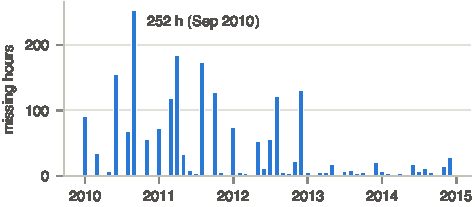
\includegraphics[width=\columnwidth]{missing.pdf}
\caption{Missing pm25 hours per month. Gaps concentrate in 2010-2012.}
\label{fig:missing}
\end{figure}

\section{Preprocessing pipeline}

\subsection{Schema and grid validation}
The loader checks the exact column list, builds a timestamp index from year, month, day and hour, and stops with an error if the hourly grid has holes or duplicates or if any weather value is missing. Later steps rely on these conditions, so the pipeline fails rather than silently repairing them.

\subsection{Decoding cumulative weather variables}
With $d_t$ the wind direction and $I_t$ the Iws value at hour $t$, the hourly wind speed is
\begin{equation}
ws_t = \begin{cases} I_t & d_t \neq d_{t-1} \\ I_t - I_{t-1} & d_t = d_{t-1} \end{cases}
\label{eq:ws}
\end{equation}
The decoded series lies in $[0.45, 20.12]$ m/s with mean 2.94; calm-variable (cv) hours average 0.99 m/s, consistent with the label. Fig.~\ref{fig:wind} shows the running total and the recovered hourly speed. The running total is kept as ws\_cum because it also encodes how long the wind has blown from one direction. Snow and rain become binary flags (snow, rain $=1$ when the counter is positive) next to the original counters.

\begin{figure}[t]
\centering
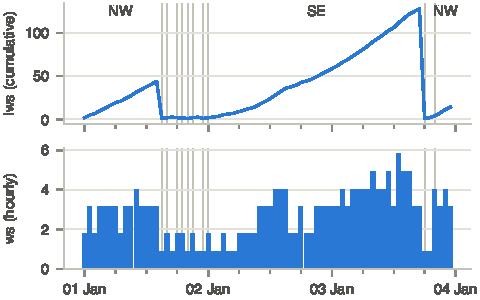
\includegraphics[width=\columnwidth]{wind_decode.pdf}
\caption{First three days of 2010. Top: raw Iws, a running total that restarts at each direction change (vertical lines; long runs labelled). Bottom: hourly speed recovered with (\ref{eq:ws}), in m/s.}
\label{fig:wind}
\end{figure}

\subsection{Wind direction encoding}
cbwd has four levels and is one-hot encoded in a fixed order (wd\_ne, wd\_nw, wd\_se, wd\_cv), so column positions do not depend on which levels appear in a fold. Unknown levels raise an error.

\subsection{Missing target values}
The label pm25 is never filled; a missing label means that hour is excluded from training loss and from evaluation. A flag pm25\_miss records the original missingness. A separate input column pm25\_in carries the last observed value forward for at most $L=3$ hours:
\begin{equation}
\tilde{y}_t = y_{t-k}, \quad k = \min\{j \ge 0 : y_{t-j}\ \text{observed}\}, \quad k \le L,
\end{equation}
and stays missing otherwise. Linear interpolation was rejected because it fills a gap using the first value after it, which leaks future information into inputs near the forecast origin. Forward filling recovers 386 input hours; \num{1681} remain missing and are left for the model stage (XGBoost handles them natively; windows for the LSTM can be dropped or masked).

\begin{figure}[t]
\centering
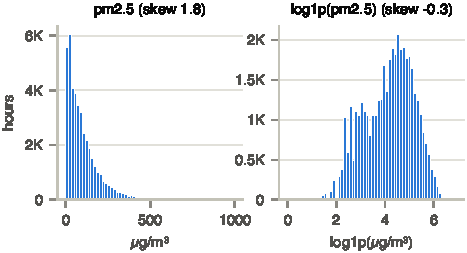
\includegraphics[width=\columnwidth]{target_hist.pdf}
\caption{Distribution of pm25 before and after log1p, 2010 to 2013.}
\label{fig:hist}
\end{figure}

\subsection{Chronological backtest folds}
Following rolling-origin evaluation \cite{tashman2000,hyndman2021}, fold $k$ evaluates on calendar year $Y_k$ and trains on all hours in $[t_0,\ s_k - G)$, where $s_k$ is 1 January of $Y_k$ and $G = 24$ hours is an embargo. With $G$ at least the forecast horizon, no training target can fall inside the evaluation year. Whole years are used so that every fold sees a full seasonal cycle. 2014 is held out as the final test year (Fig.~\ref{fig:folds}, Table~\ref{tab:folds}).

\begin{figure}[t]
\centering
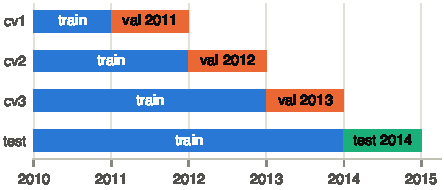
\includegraphics[width=\columnwidth]{folds.pdf}
\caption{Expanding-window folds. The 24-hour embargo before each evaluation year is too short to see at this scale.}
\label{fig:folds}
\end{figure}

\begin{table}[t]
\centering
\caption{Fold sizes (hours)}
\label{tab:folds}
\begin{tabular}{@{}lllrr@{}}
\toprule
Fold & Train until & Evaluate & Train & Labelled eval \\
\midrule
cv1 & 2010-12-30 23:00 & 2011 & \num{8736} & \num{8032} \\
cv2 & 2011-12-30 23:00 & 2012 & \num{17496} & \num{8295} \\
cv3 & 2012-12-30 23:00 & 2013 & \num{26280} & \num{8678} \\
test & 2013-12-30 23:00 & 2014 & \num{35040} & \num{8661} \\
\bottomrule
\end{tabular}
\end{table}

\subsection{Leak-free scaling}
For each fold a scaler is fitted on that fold's training rows only and saved to disk:
\begin{equation}
z = \frac{g(x) - \mu_{\text{train}}}{\max(\sigma_{\text{train}}, \epsilon)},
\end{equation}
where $g$ is log1p for the skewed columns (pm25, pm25\_in, ws, ws\_cum, snow\_cum, rain\_cum, all with skewness above 1) and the identity otherwise. Tree models can ignore it; recurrent models use it, and predictions are mapped back to \si{\micro\gram\per\cubic\metre} with the inverse transform before computing MAE, RMSE and $R^2$.

\section{Implementation and verification}
The pipeline is a Python package (src/aqf/data) driven by one configuration file (configs/data.yaml) and run with \texttt{python -m aqf.data.pipeline}. It writes the cleaned hourly frame (data/interim/hourly.parquet), the fold boundaries (data/processed/folds.json), one scaler per fold (data/processed/scalers) and the audit numbers used in this report (reports/preprocessing/qa.json). Nine tests check that: the grid is complete and hourly; only the target is missing; summing decoded speeds within each direction run rebuilds Iws exactly; the one-hot columns are exclusive; the label is unchanged and the flag matches it; filling at hour $t$ is identical whether or not later hours exist (causality); folds never overlap and respect the embargo; scaler statistics do not change when evaluation rows are altered; and the scaler round-trips through disk and its inverse.

\section{Next steps}
Feature engineering (lags, rolling means and calendar terms, built after sorting by time), the persistence and seasonal-naive baselines, and the XGBoost model build on these outputs. The audit suggests a 24-hour seasonal-naive baseline rather than a weekly one, since PM2.5 autocorrelation is 0.40 at lag 24 but 0.02 at lag 168. The forecast horizon and the AQI standard still have to be fixed and stated.

\begin{thebibliography}{1}
\bibitem{uci} S. Chen, ``Beijing PM2.5,'' UCI Machine Learning Repository, 2015, doi: 10.24432/C5JS49.
\bibitem{liang2015} X. Liang, T. Zou, B. Guo, S. Li, H. Zhang, S. Zhang, H. Huang, and S. Chen, ``Assessing Beijing's PM2.5 pollution: severity, weather impact, APEC and winter heating,'' \emph{Proc. Royal Society A}, 2015.
\bibitem{hyndman2021} R. J. Hyndman and G. Athanasopoulos, \emph{Forecasting: Principles and Practice}, 3rd ed. Melbourne, Australia: OTexts, 2021.
\bibitem{tashman2000} L. J. Tashman, ``Out-of-sample tests of forecasting accuracy: an analysis and review,'' \emph{Int. J. Forecasting}, vol. 16, no. 4, pp. 437--450, 2000.
\bibitem{bergmeir2012} C. Bergmeir and J. M. Ben\'{i}tez, ``On the use of cross-validation for time series predictor evaluation,'' \emph{Information Sciences}, vol. 191, pp. 192--213, 2012.
\end{thebibliography}

\end{document}
